\newpage
\chapter{Trabajo de investigación}

\subsubsection{Investigar}

Investigar sobre uno de estos tres temas:

\begin{enumerate}
  \item \textbf{DCA con submuestreo}
  \item \textbf{Diseño Cuadrado Latino}
  \item \textbf{Diseño Greco Latino}
\end{enumerate}

Presente un informe académico de alguno de los temas elegidos, este informe debe tener fundamentos teóricos, aplicaciones y un ejercicio resuelto paso a paso usando las sumas de cuadrados (descomponiendo la variabilidad total), y corroborado en el R; Verificar los supuestos del modelo en el R, (utilizar transformaciones si fuera necesario) Así mismo si es pertinente usar pruebas de comparación múltiple.

\subsubsection{Componentes mínimo del informe}

\begin{itemize}
  \item[a)] Presente el modelo aditivo lineal y explique sus componentes según el enunciado de la pregunta.
  \item[b)] Aplicaciones.
  \item[c)] Enunciado del ejemplo (cite o link) 
  \item[d)] Anova (paso a paso)
  \item[e)] comprobación con el R
  \item[f)] Comprobación de supuestos, (Transformar si es necesario)
  \item[g)] Comparaciones multiples
\end{itemize}

\subsubsection{Indicaciones finales}

\begin{itemize}
  \item[a)] El documento debe utilizar un lenguaje académico.
  \item[b)] Subir el informe final-documento en pdf.
  \item[c)] Subir el Script y data comprimido (se descontaran puntos si no lo hace).
  \item[d)] Subir tu informe antes de las 23:59 pm (18-09-2025)
\end{itemize}

\section{SOLUCIÓN}

Para realizar la resolución de esta activad se esta usando el editor de texto \LaTeX en el cual se hizo las debidas configuraciones en el preámbulo para obtener resultados en formato APA, me decidí por buscar el caso del diseño cuadrado latino.

\subsection{Diseño en cuadrados latinos}

\subsubsection{Introducción}

En este modelo se consideran simultáneamente dos variables de bloque \citep{ugr_latinos}. Por ejemplo considera un experimento en el que se quiere estudiar el efecto de distintos tipos de semilla en el rendimiento del trigo y se considera que en el rendimiento puede influir los tipos de abonos e insecticidas empleados. Se puede trabajar con un diseño completo aleatorizado donde el factor es el tipo de semilla y las variables de bloques son los tipos de abono e insecticida.

Pero su inconveniente es el de requerir excesivas unidades para su realización, para estos tres factores se tengan $K_1$, $K_2$ y $K_3$ niveles en cada uno de los factores de lo que requeriría $K_1 \times K_2 \times K_3$ unidades experimentales por lo que pueden resultar muy costos. Entonces se recurre a un tipo especial de diseño en bloques incompletos aleatorizados en el que se selecciona una parte del diseño completo de tal forma que se puedan estimar los efectos de interés.

Uno de estos bloques es el modelo en cuadrado latino el cual requiere el mismo número de niveles para los tres factores.

\subsubsection{Descripción del modelo}

En estos diseños el número de niveles del factor principal tiene que coincidir con el número de niveles de las dos variables de bloque o factores secundarios y además hay que suponer que no existe interacción entre ninguna pareja de factores.

Suponiendo que el número de niveles de cada uno de los factores es $K$. El diseño cuadrado latino utiliza $K^2$ bloques, cada bloque corresponde a una de las posibles combinaciones de niveles de los dos factores de control. En cada bloque se aplica un solo tratamiento de manera que cada tratamiento debe aparecer con cada uno de los niveles de los dos factores de control.

Para el caso de abonos donde se tienen para la semilla, abono e insecticidad con $K=4$ niveles se muestra la siguiente tabla:

\begin{figure}[h!]
    \begin{tcolorbox}[colback=white, colframe=black, boxrule=1.5pt, sharp corners=all]
          \begin{center}
            {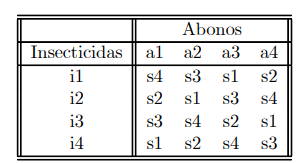
\includegraphics[scale=1.5]{images/img1.png}}
          \end{center}
        \end{tcolorbox}
\end{figure}

De donde un diseño cuadrado latino tiene las siguientes características:

\begin{enumerate}
  \item Se controlan tres fuentes de variabilidad, un factor principal y dos factores de bloque.
  \item Cada uno de los factores tiene el mismo número de niveles, $K$.
  \item Cada nivel del factor principal aparece una sola vez en cada fila y una vez en cada columna.
  \item No hay interacción entre los factores.
\end{enumerate}

\subsubsection{Planteamiento del modelo}

En un diseño en cuadrado latino intervienen los siguientes factores: un factor principal y dos factores secundarios o variables de bloque. Se supone que no existe interacción entre estos tres factores, teniendo un modelo aditivo.

Si consideramos que los tres factores son de efectos fijos, el modelo estadístico para este diseño es:

$$
y_{ijh} = \mu + {\tau}_{i} + {\beta}_{j} + {\gamma}_{h} + {\epsilon}_{ijh}
$$

En el que $i=j=h= (1, 2, \cdots , K )$ y donde:

\begin{itemize}
  \item ${y}_{ijh}$: Representa la observación correspondiente de la $i$-ésima fila, $j$-ésima columna y $h$-ésima letra latina.
  \item $\mu$: Es la media global.
  \item $\tau_i$: Es el efecto producido por el $i$-ésimo nivel del factor fila. Los cuales están sujetos a la restricción $\sum {\tau}_{i} = 0$
  \item ${\beta}_{j}$: Es el efecto producido por el $j$-ésimo nivel del factor columna. Dichos efectos están sujetos a la restricción $\sum {\beta}_{j} = 0$
  \item ${\gamma}_{h}$: Es el efecto producido por la $h$-ésima letra latina. Dichos efectos están sujetos a la restricción $\sum {\gamma}_{h} = 0$
  \item ${\epsilon}_{ijh}$: Son los errores que siguen una distribución $N \sim (0,\sigma)$
\end{itemize}

\subsubsection{Ejemplo}

Se ha realizado el experimento aleatorio correspondiente y se designó por las letras (A, B, C, D) a los tratamientos. Así, el cuadrado latino resultante junto con las observaciones obtenidas, dan lugar a la siguiente tabla

\begin{figure}[H]
    \begin{tcolorbox}[colback=white, colframe=black, boxrule=1.5pt, sharp corners=all]
          \begin{center}
            {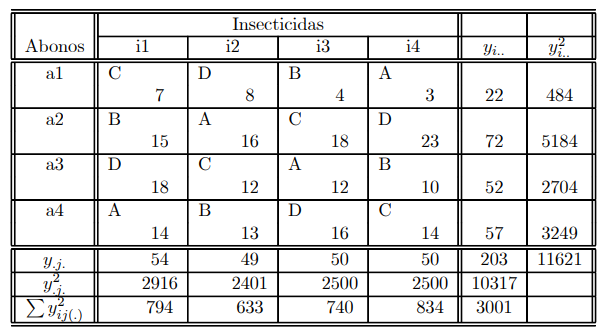
\includegraphics[scale=1]{images/img2.png}}
          \end{center}
        \end{tcolorbox}
\end{figure}

Asi mismo la suma de cuadrados para el análisis de la varianza

\begin{figure}[H]
    \begin{tcolorbox}[colback=white, colframe=black, boxrule=1.5pt, sharp corners=all]
          \begin{center}
            {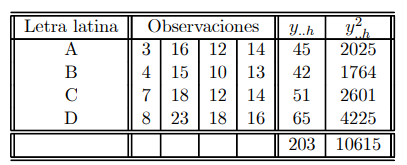
\includegraphics[scale=1.5]{images/img3.png}}
          \end{center}
        \end{tcolorbox}
\end{figure}

$$
SCT = \sum_{i=1}^{4} \sum_{j=1}^{4} {y}_{ij.}^{2} - \frac{{y}_{\ldots}^{2}}{K^2} = 3001 - \frac{203^2}{4^2} = 425.4375
$$

$$
SCF = \frac{1}{K} \sum_{i=1}^{4}{y}_{i..}^{2} - \frac{{y}_{\ldots}^{2}}{K^2} = \frac{11621}{4} - \frac{203^2}{4^2} = 329.6875
$$

$$
SCC  = \frac{1}{K}\sum_{j=1}^{4}{y}_{.j.}^{2} - \frac{{y}_{\ldots}^{2}}{K^2} = \frac{10317}{4} - \frac{203^2}{4^2} = 3.6875
$$

$$
SCL  = \frac{1}{K}\sum_{h=1}^{4}{y}_{..h}^{2} - \frac{{y}_{\ldots}^{2}}{K^2} = \frac{10615}{4} - \frac{203^2}{4^2} = 78.1875
$$

Y la suma de cuadrados del error se obtiene por diferencia

$$
SCR = SCT - SCF - SCC - SCL = 13.875
$$

En el que la tabla ANOVA seria el siguiente

\begin{figure}[H]
    \begin{tcolorbox}[colback=white, colframe=black, boxrule=1.5pt, sharp corners=all]
          \begin{center}
            {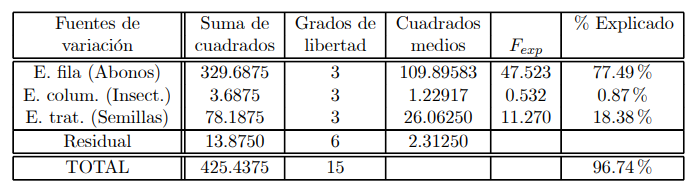
\includegraphics[scale=1]{images/img4.png}}
          \end{center}
        \end{tcolorbox}
\end{figure}

Realizando el contraste al $5\%$ y tomamos el $F_{cal}$ con el $F_{teo}$.Se concluye que los efectos de los abonos y semillas son significativas, pero no de los insecticidas.

Por última veamos la aplicación de los resultados en RStudio.

\begin{figure}[h!]
        \begin{tcolorbox}[colback=white, colframe=black, boxrule=1.5pt, sharp corners=all]
            {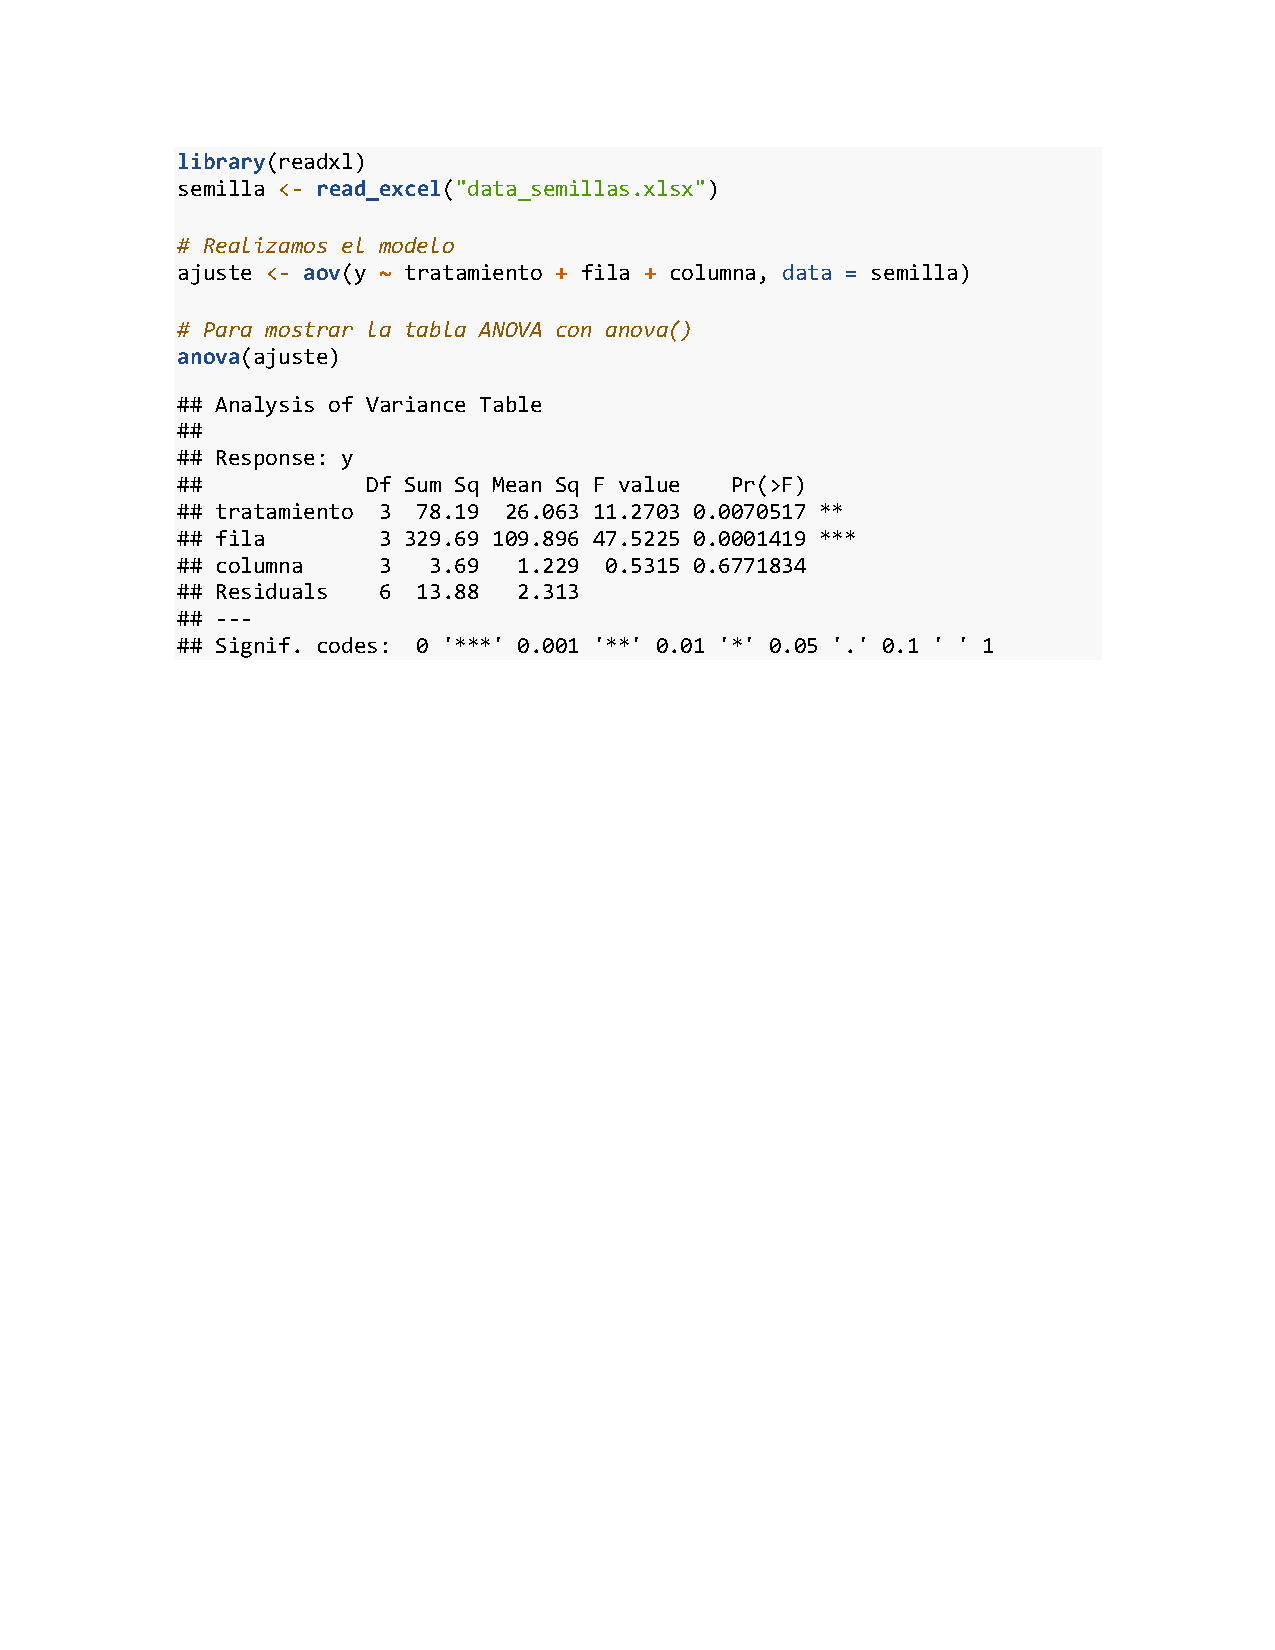
\includegraphics[width=\linewidth, height=8cm, trim=2.5cm 16cm 2.5cm 2.5cm, clip]{images/imgscript.pdf}}
        \end{tcolorbox}
\end{figure}
